\section{R2U2 Software Implementation in C Programming}
The C version of R2U2 has two modes of operation: an offline mode and an online mode. The offline mode functions similar to the Python implementation of R2U2: it provides an offline verification of a trace or it can be used to validate an MLTL formula over a trace. Additionally, this offline mode allows developers to perform regression testing over a variety of benchmark traces \& formulas to make sure updates did not break the tool. The online version is intended to be versatile; it can be run either on an embedded platform or a personal computer. Note that this online version requires the sensor values R2U2 is reasoning over to be continuously written into a file structure, which means that the embedded platform must support writing to a file.

\subsection{Getting Started}
Note that the following must be installed to use the C implementation of R2U2:
\begin{itemize}
	\item \textbf{Python:} Version 3.6 (or greater)
	\item \textbf{Python Packages:} ply
	\item \textbf{Unix Packages:} pkg-config, fftw3
\end{itemize}
\subparagraph{R2U2 Tool-chain Flow:} Figure \ref{fig:r2u2cflow} shows the flow of the C version of R2U2. To use this version of R2U2, the user needs to supply R2U2 with a trace file (\textit{.trc}) and an MLTL formula. The user starts by converting the MLTL formula into an Assembly File (\textit{.ftasm}). Within this step, the SCQ size (amount of memory required for R2U2's instruction sequence) is determined and stored in a \textit{.ftscq} file. The second step is to take this \textit{.ftasm} assembly file and convert it into a Binary Instruction (\textit{.ftm}) and an Binary Instruction Interval (\textit{.fti}). Lastly, the user specifies their \textit{.ftm}, \textit{.fti}, \textit{.ftscq}, and their own \textit{.trc} file to R2U2, via a UNIX command line. R2U2 compiles this information and begins its online or offline execution. The results of R2U2 are displayed through the command terminal and logged into a \textit{.log} file within the \textbf{R2U2\_SW/R2U2\_C} directory.

\begin{figure}[H]
	\begin{center}
	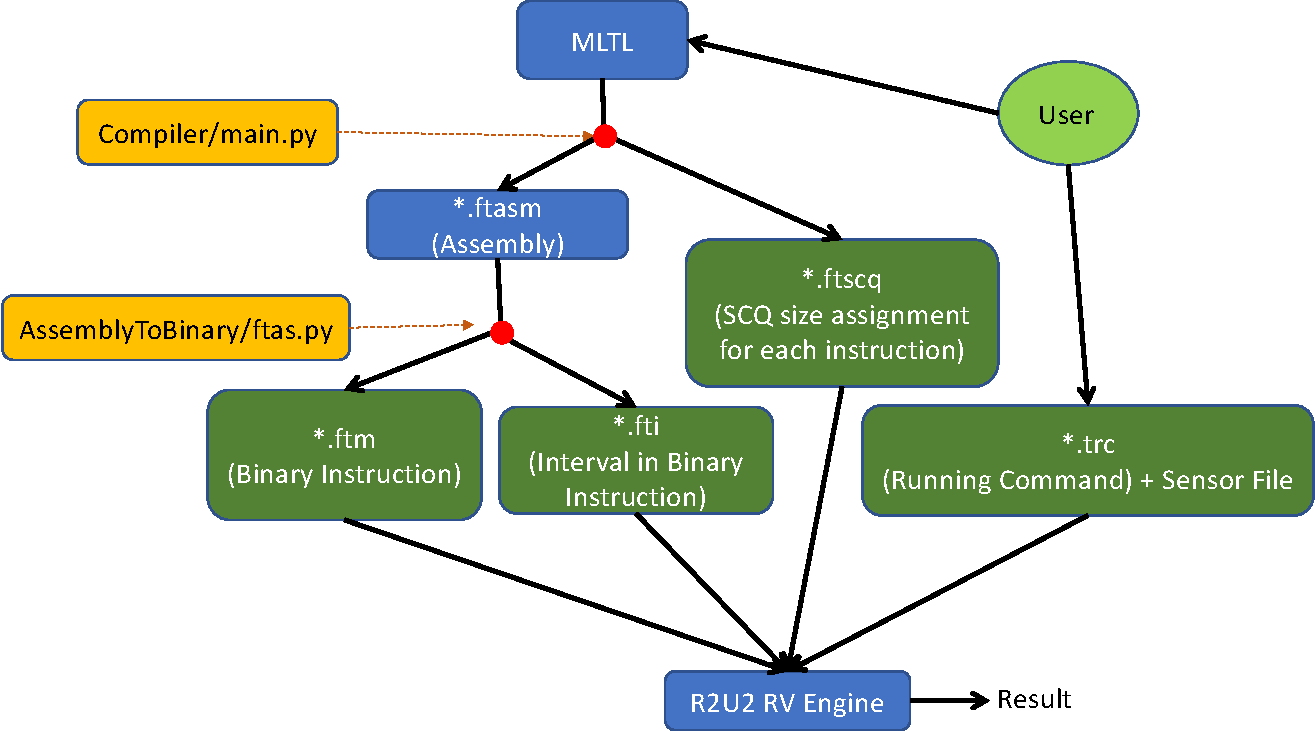
\includegraphics[scale=0.5]{fig/r2u2_c_flow.pdf}
	\caption{Flow of how the C version of R2U2 is compiled and deployed. 
	\label{fig:r2u2cflow}} 
	\end{center}
\end{figure}

The C version of R2U2 must be executed from a UNIX based command line interface (CLI). Described below are the file types that the user must supply to run R2U2:
\begin{itemize}
	\item \textbf{MLTL Formula:} This is the MLTL formula R2U2 will reason over. This formula can be either directly entered into the CLI or saved into the \textit{main.py} file within the \textbf{/tools/Compiler/} directory of R2U2. More detail into the syntax of the MLTL formula will be described in Section \ref{mltlFormula}. 
	\item \textbf{Trace File:} This file contains the sensor values R2U2 will reason over. Note that there will be two different formats for this file depending on whether R2U2 will be run offline or online. More detail into the two file formats, the syntax, and how to convert these sensor values into Boolean atomics will be discussed in Section \ref{TraceFile}.
\end{itemize}

\subsection{File Formats}
\label{FileFormats}
This version of R2U2 has two input parameters: an MLTL formula and a trace file. This section describes the syntax \& structure for theses files and how a user would incorporate them into the current R2U2 structure.

\subsubsection{MLTL Formula}
\label{mltlFormula}
The MLTL formula that R2U2 will reason over must be implemented in one of two ways: either written and saved into the \textit{main.py} file (located within the \textbf{tools/Compiler} directory) or entered directly into the CLI when compiling the \textit{.ftasm} assembly file. In either case the syntax for the MLTL formula is identical and can be seen in Table \ref{mltlFormulaTable}. Note that the only difference is how special characters are labeled in the CLI: they must be proceeded with a `` $\setminus$ ''. Additionally, the syntax for the MLTL formulas can be seen in Table \ref{syntaxMLTL}.

\begin{table}[H]
	\caption{An example of an MLTL formula and the syntactical conversion into either the file type or the CLI.}
	\label{mltlFormulaTable}
	\begin{center}
	\begin{tabular}{l | l}
		\hline
		\hline
		\textbf{Type} & \textbf{Formula Format}\\
		\hline
		Expression & $G_{0,3}((a_0\bigwedge a_1)\bigwedge (a_2 \bigwedge s_3))$\\
		\textit{main.py} & MLTL = ``G[0,3]((a0 \& a1) \& (a2 \& a3))''\\
		CLI & G[0,3]((a0$\setminus$\&a1) $\setminus$\&(a2$\setminus$\&a3))\\
		\hline
		\hline
	\end{tabular}
	\end{center}
\end{table}

%\begin{table}[H]
%	\caption{The format for the MLTL operators, which are used to create a single MLTL formula which can either be saved to the \textit{main.py} file or incorporated into the CLI. Note that $E$1 and $E$2 denote that that parameter can be either an expression, to allow for more complex formulas, or a single atomic.}
%	\label{syntaxMLTL}
%
%	\begin{center}
%	\begin{tabular}{l | c | c | c | c | c | c}
%		\hline
%		\hline
%		\textbf{Expression} & \textit{NOT} & \textit{Next} & \textit{Until} & \textit{Global} & \textit{AND} & \textit{OR}\\
%		\hline
%		\textbf{Syntax} & !$E$1 & $XE$1 & $E$1 $U$[$t_i$,$t_f$] $E$2 & $G$[$t_i$,$t_f$] $E$1 & $E$1 \& $E$2& $E$1 $|$ $E$2\\
%		\hline
%		\textbf{Precedence} & 1 & 1 & 2 & 2 & 3 & 3\\
%		\hline
%		\hline
%	\end{tabular}
%	\end{center}
%\end{table}

\begin{table}[H]
	\label{syntaxMLTL}

	\begin{center}
	\begin{tabular}{l | c  }
		\hline
		\hline
		\textbf{Expression} & \textit{Syntax} \\
		\hline
		Negation     & \texttt{!E1} \\
		Conjunction  & \texttt{E1 \& E2}\\
		Disjunction  & \texttt{E1 | E2} \\
		Implication  & \texttt{E1 -> E2} \\
		Equivalence  & \texttt{E1 <-> E2}\\
		\hline
		Globally     & \texttt{G[ti,tf] E1} or \texttt{G[tf] E1} \\
		Future       & \texttt{F[ti,tf] E1} or \texttt{F[tf] E1}\\
		Until        & \texttt{E1 GU[ti,tf] E2} or \texttt{E1 U[tf] E2} \\
		\hline
		Historically & \texttt{H[ti,tf] E1} or \texttt{H[tf] E1} \\
		Once         & \texttt{O[ti,tf] E1} or \texttt{O[tf] E1} \\ 
		Since        & \texttt{E1 S[ti,tf] E2} or \texttt{E1 S[tf] E2} \\
		\hline
		\hline
	\end{tabular}
	\end{center}
\end{table}

\subsubsection{Trace File}
\label{TraceFile}
In addition to the MLTL formulas, users need to supply a time series of sensor data, i.e., a trace file. There are two different formats for this file: one for the offline version and one for the online. Both versions are described in Table \ref{SensorFileTable}.

\begin{table}[H]
	\caption{Examples of the format for the \textit{.trc} Trace Files}
	\label{SensorFileTable}
	\begin{center}
	\begin{tabular}{l | ccc | cccc}
		\hline
		\hline
		\textbf{File Type} & \multicolumn{3}{c|}{\textbf{Offline \textit{.trc} File}} & \multicolumn{4}{c}{\textbf{Online \textit{.trc} File}}\\
		\hline
		Line \# & Sensor 0 & Sensor 1 & $\dots$ & Command & Sensor 0 & Sensor 1 & $\dots$\\
		\hline
		line 1 & 1002 &  9.9 & $\dots$ & \textbf{i} & 1002 &  9.9 & $\dots$\\
		line 2 & 1005 & 10.0 & $\dots$ \\
		line 3 & 1011 &  9.8 & $\dots$ \\
		line 4 & 1015 & 10.4 & $\dots$ \\
		line 5 & $\vdots$ & $\vdots$ & \\
		\hline
		\hline
	\end{tabular}
	\end{center}
\end{table}
Note that the online version's trace file must be written on each time stamp. Additionally, a command structure is introduced in the first column of the online \textit{.trc} file to allow R2U2 to initialize, increment the time stamp, and to terminate execution. The values of these commands are as follows:
\begin{itemize}
	\item \textbf{i = -2:} Terminate the current execution.
	\item \textbf{i = -1:} Reset R2U2 to its initial state.
	\item \textbf{i $\geq$ 0:} The time stamp for R2U2 (starting at i = 0).
\end{itemize}

In addition to providing the trace file, the user must specify how the sensor inputs will be converted into Boolean atomics. The \textbf{at\_checkers\_update} function  within the \textit{at\_conversion.c} file must be modified to perform this conversion. This file is contained within the \textbf{R2U2\_SW/R2U2\_C/src/AT/} directory. Figure \ref{fig:atConversion} shows the \textit{at\_conversion.c} function with an example conversion of $\textit{Sensor 0}<1000$, $\textit{Sensor 0}>950$, $\textit{Sensor 1}>9.5$, and $\textit{Sensor 1}<10.0$.

\begin{figure}[H]
	\begin{center}
		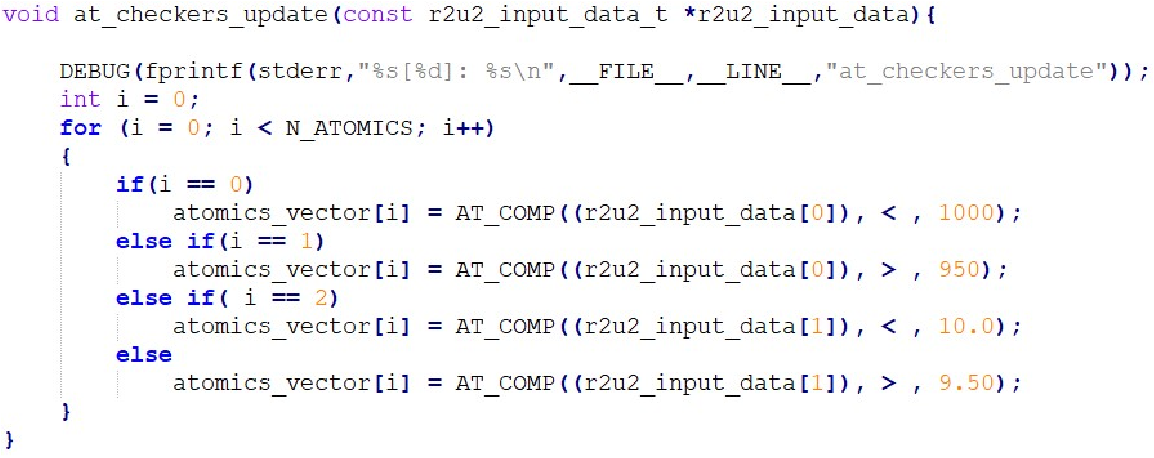
\includegraphics[scale=0.5]{fig/ATconversionScreenshot.pdf}
		\caption{A screenshot of the \textbf{at\_checkers\_update} function within the \textit{at\_conversion.c} file. Note that this function must be modified in order to convert the sensor values into boolean atomics.
		\label{fig:atConversion}}
	\end{center}
\end{figure}

\subsection{Running R2U2 - C Version}
\label{R2U2c}


\subsubsection{Offline Execution Steps}
\label{OfflineC}
\begin{enumerate}
	\item Navigate to the \textbf{../R2U2\_SW/R2U2\_C/} directory
	\item In a UNIX bash terminal, compile the project using the command
	\begin{lstlisting}[language=C]
	make
	\end{lstlisting}
	\item Modify the \textbf{at\_conversion.c} function to convert the sensors into boolean atomics.
	\item Navigate backwards to the \textbf{tools} directory via 
	\begin{lstlisting}[language=C]
	cd ../../tools
	\end{lstlisting}
	\item Next, the \textit{.ftasm} \& the \textit{.ftscq} files must be complied. There are two ways to proceed, depending on how the user wishes to input the MLTL formula:
	\begin{enumerate}
		\item \textbf{main.py:} Execute the command
		\begin{lstlisting}[language=C]		
		python Compiler/main.py
		\end{lstlisting}
		\item \textbf{CLI:} Execute the command
		\begin{lstlisting}[language=C]
		python Compiler/main.py [MLTL Formula]
		\end{lstlisting}
	\end{enumerate}
	\item Compile the \textit{.ftm} \& \textit{.fti} files from the newly generated \textit{.ftasm} using the command:
	\begin{lstlisting}[language=C]
	cat tmp.ftasm | python AssemblyToBinary/ftas.py tmp
	\end{lstlisting}
	\item Navigate back to the \textbf{R2U2\_C} directory via
	\begin{lstlisting}[language=C]
	cd ../R2U2_C
	\end{lstlisting}
	\item Begin R2U2's execution with the following command:
	\begin{lstlisting}[language=C]
	./bin/r2u2 [location of .trc file, from current directory] 
	[location of the .ftm file] [location of the .fti file] 
	[location of the .ftscq file]
	\end{lstlisting}

\end{enumerate}

\subsubsection{Online Execution Steps}
\label{OnlineC}


\clearpage
